% Document
\documentclass{article}

% Packages
\usepackage[utf8]{inputenc}                                                             % input encoding
\usepackage[T1]{fontenc}                                                                % font encoding
\usepackage[ngerman]{babel}                                                             % for German
\usepackage[left=2cm, right=2cm, top=2.5cm,bottom=2.5cm]{geometry}                      % for page size
\usepackage{natbib}                                                                     % for bibliography
\usepackage{graphicx}                                                                   % for images
\usepackage[font=normal,labelfont=bf,textfont=rm,position=bottom,skip=10pt]{caption}    % for captions
\usepackage{amsmath}                                                                    % for formulas
\usepackage{float}                                                                      % for images at right position
\usepackage[autostyle=true,german=quotes]{csquotes}                                     % for proper quotes
\usepackage{siunitx}                                             

% for MATLAB-codes
\usepackage{comment}
\usepackage{bm}
\usepackage{subfigure}
\usepackage{hyperref}
\usepackage{pdfpages} %fuer einfuegen von PDFs (Aufgabenstellung)
% for block comments

\bibliographystyle{agsm}

\newcommand{\geodaten}[1]{\underline{#1}}     % Vektor als Matrix

% Document start
\begin{document}
\section{Bahnintegration}
Da dünne Luft in LEO Bereich existiert, bremsen die Objekten sich langsam und sie werden am Ende auf die Erde fallen. Allerdings kommt dann die Frage: wie lang dauert dieser Prozess?
\\\\
\autoref{eq2} beschriebt die atmosphärische Widerstand des Objekts im Raum. $A$ ist die Querschnittfläche entlang Geschwindigkeitsrichtung, $m$ ist die Masse, $\rho$ ist die Atmosphärendichte, $\bm{\dot{r}_a}$ und $\bm{\dot{r}}$ sind jeweils die Geschwindigkeit der Atmosphäre und Objekt. $C_d$ beschreibt die Form des Objekts im Raum, typische Werte sind bspw. 1 für Kugel und ca. 2.5 für ISS(Internationale Raum Station).
\begin{equation}\label{eq2}
	\frac{\bm{f}_{atm}}{m} = -\frac{1}{2} \cdot C_d \cdot \rho \cdot \frac{A}{m} \cdot \left(\bm{\dot{r}} - \bm{\dot{r}_a}\right) \cdot |\bm{\dot{r}} - \bm{\dot{r}_a}|
\end{equation}
Das bedeutet, bevor wir die Bahnintegration implementieren, müssen wir zunächst Raumobjekten bzw. Raumatmosphäre untersuchen.
\subsection{Atmosphärische Eigenschaft im Raum}
2 Atmosphäre Modelle sind untersucht nämlich Harris-Priester Modell \cite{harris1963relation} und MSIS-E-00\cite{picone2002nrlmsise}. Bei Harris-Priester Model ist die Atmosphärische Dicht nur von Höhe abhängen und MSIS-E-00 ist ein viel präziseres Modell, bei dem geographische Ort, Höhe und auch Zeit eine Rolle spielen.
\\\\
Bei MSIS-E-00 Model ist die Atmosphärische Dichte von mehre Parametern abhängen, bspw.  ellipsoidische Höhe, Länge, Breite und Zeit. In \autoref{fig:msise00_400km} sind die atmosphärische Dichte \SI{400}{\kilo \meter}
\begin{figure}[ht]\centering 
	\subfigure[]{
		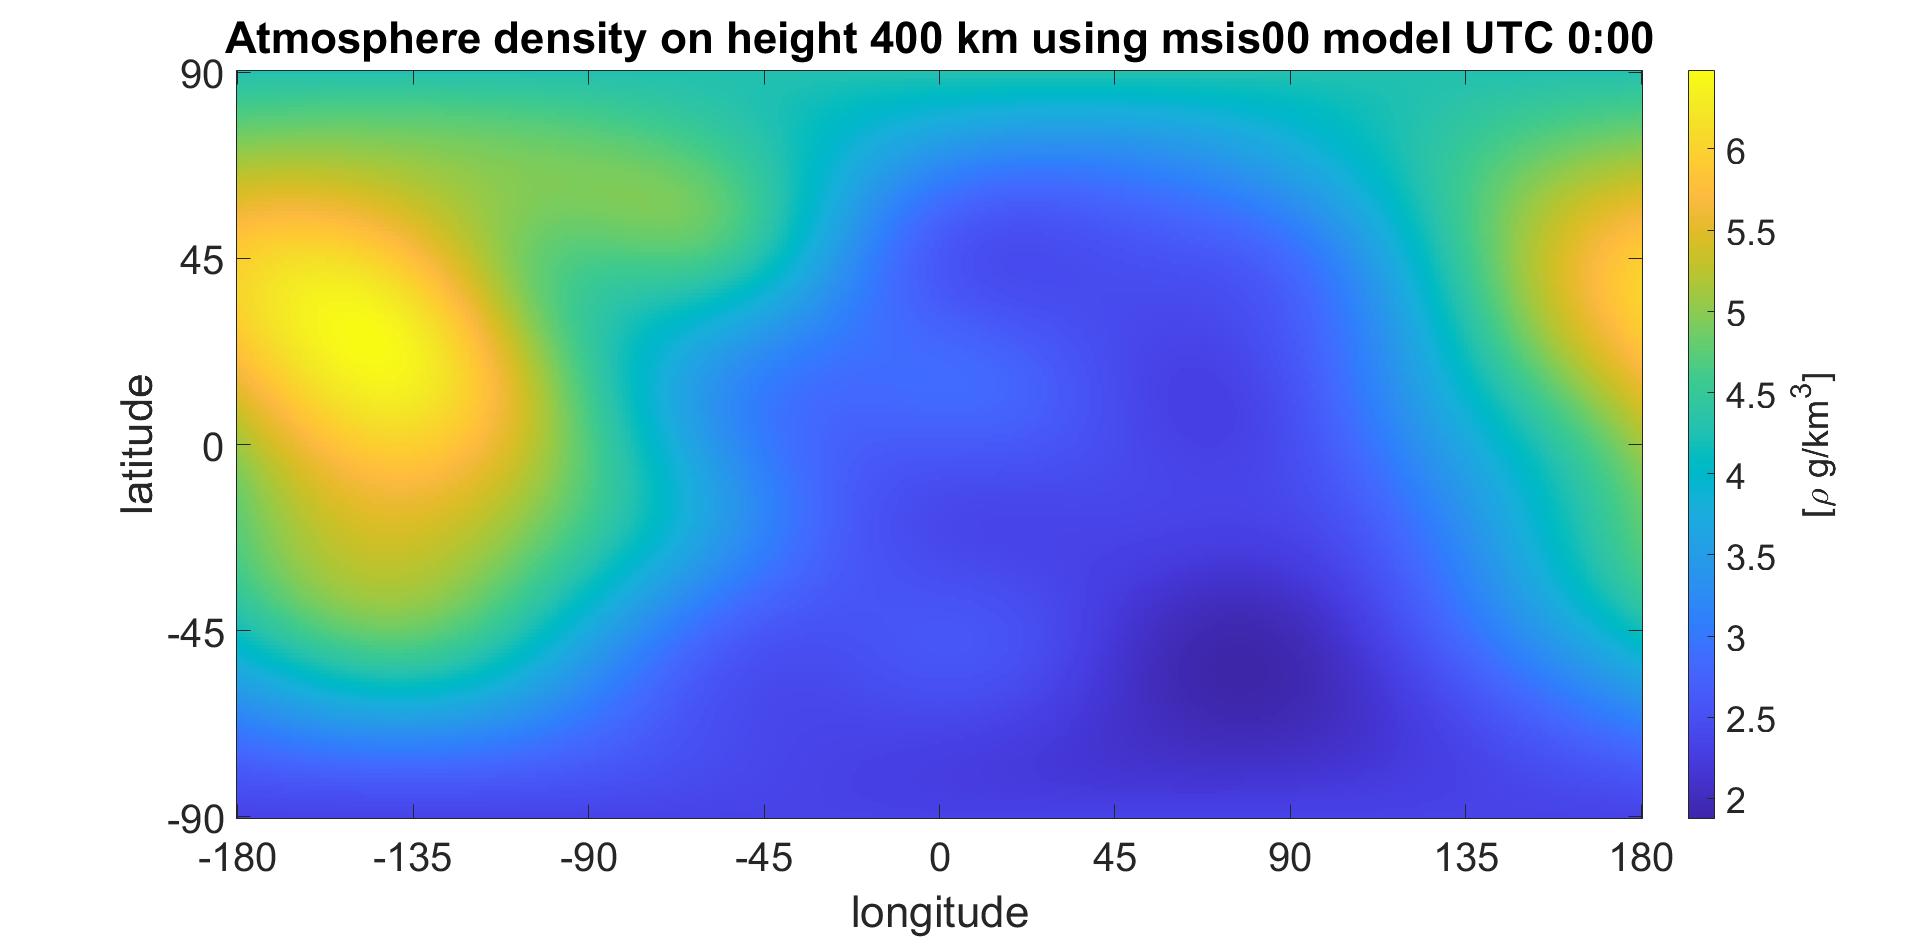
\includegraphics[width=0.9\textwidth]{images/msis_day.png}}
	\subfigure[]{
		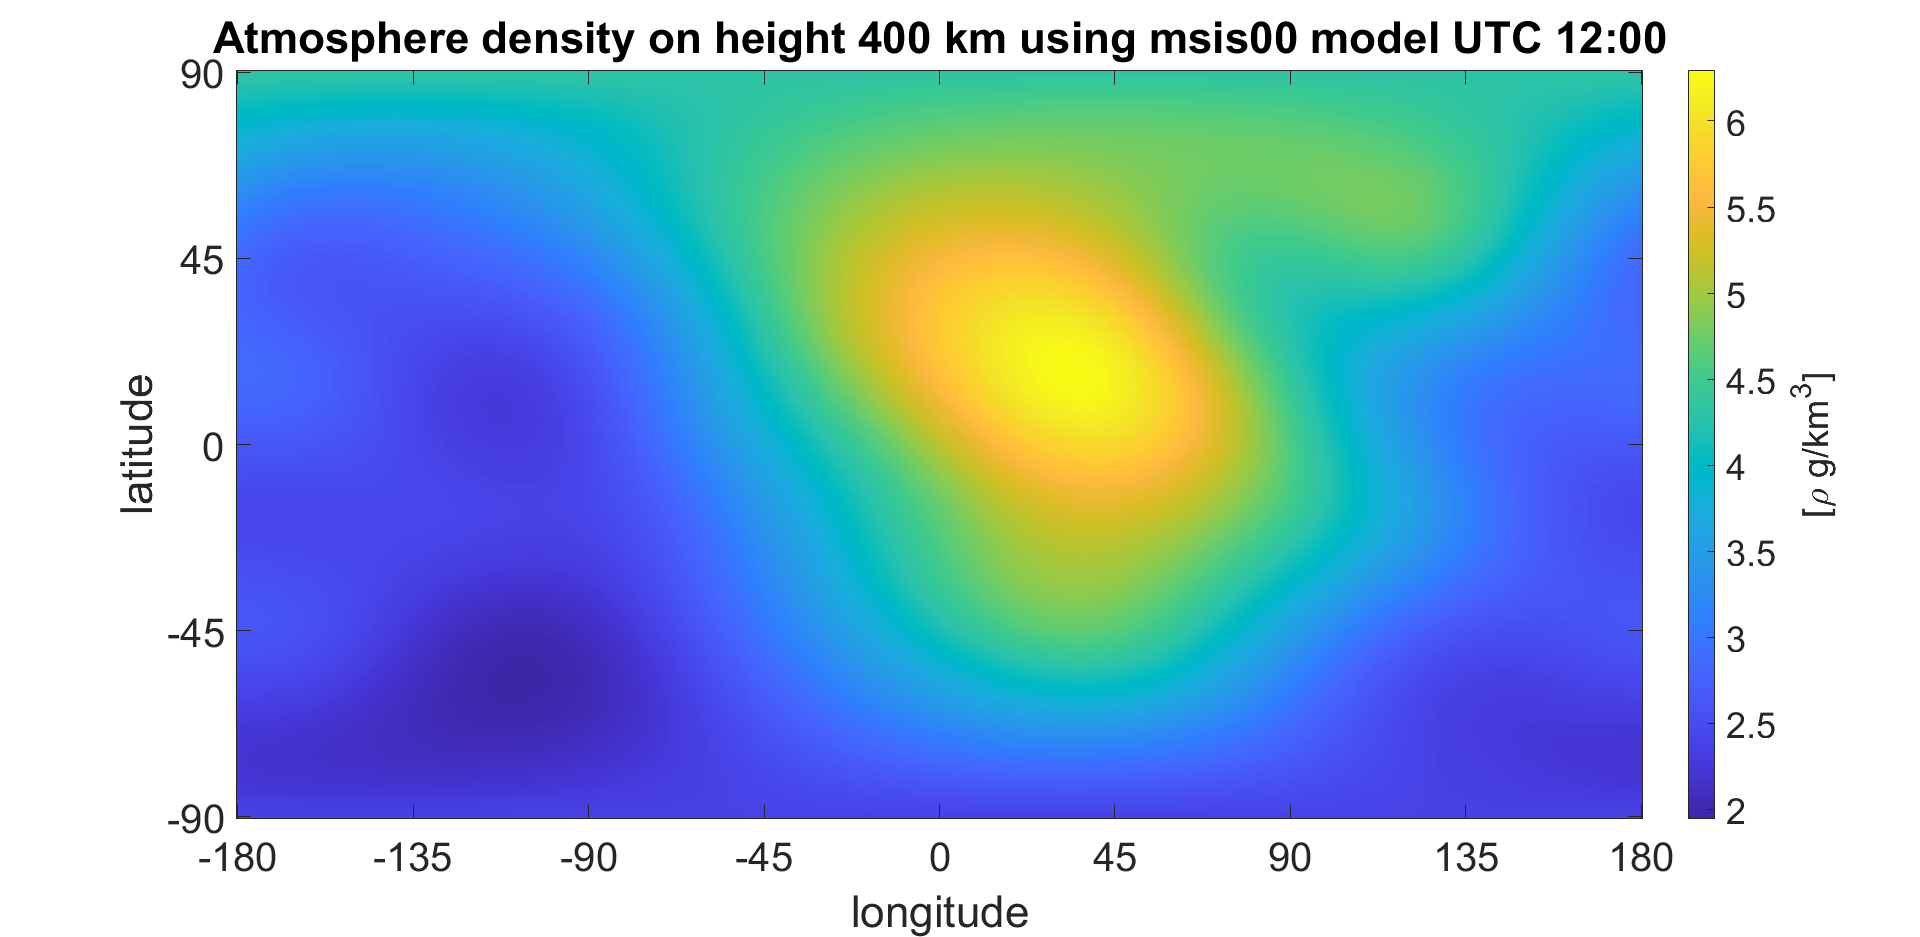
\includegraphics[width=0.9\textwidth]{images/msis_night.png}}
	\caption{Atmosphärische Dichte \SI{400}{\kilo \meter} über die Erde um 0:00 und 12:00 UTC}
	\label{fig:msise00_400km}
\end{figure}


\begin{figure}[ht]\centering \label{fig:compare_model}
	\subfigure[]{
		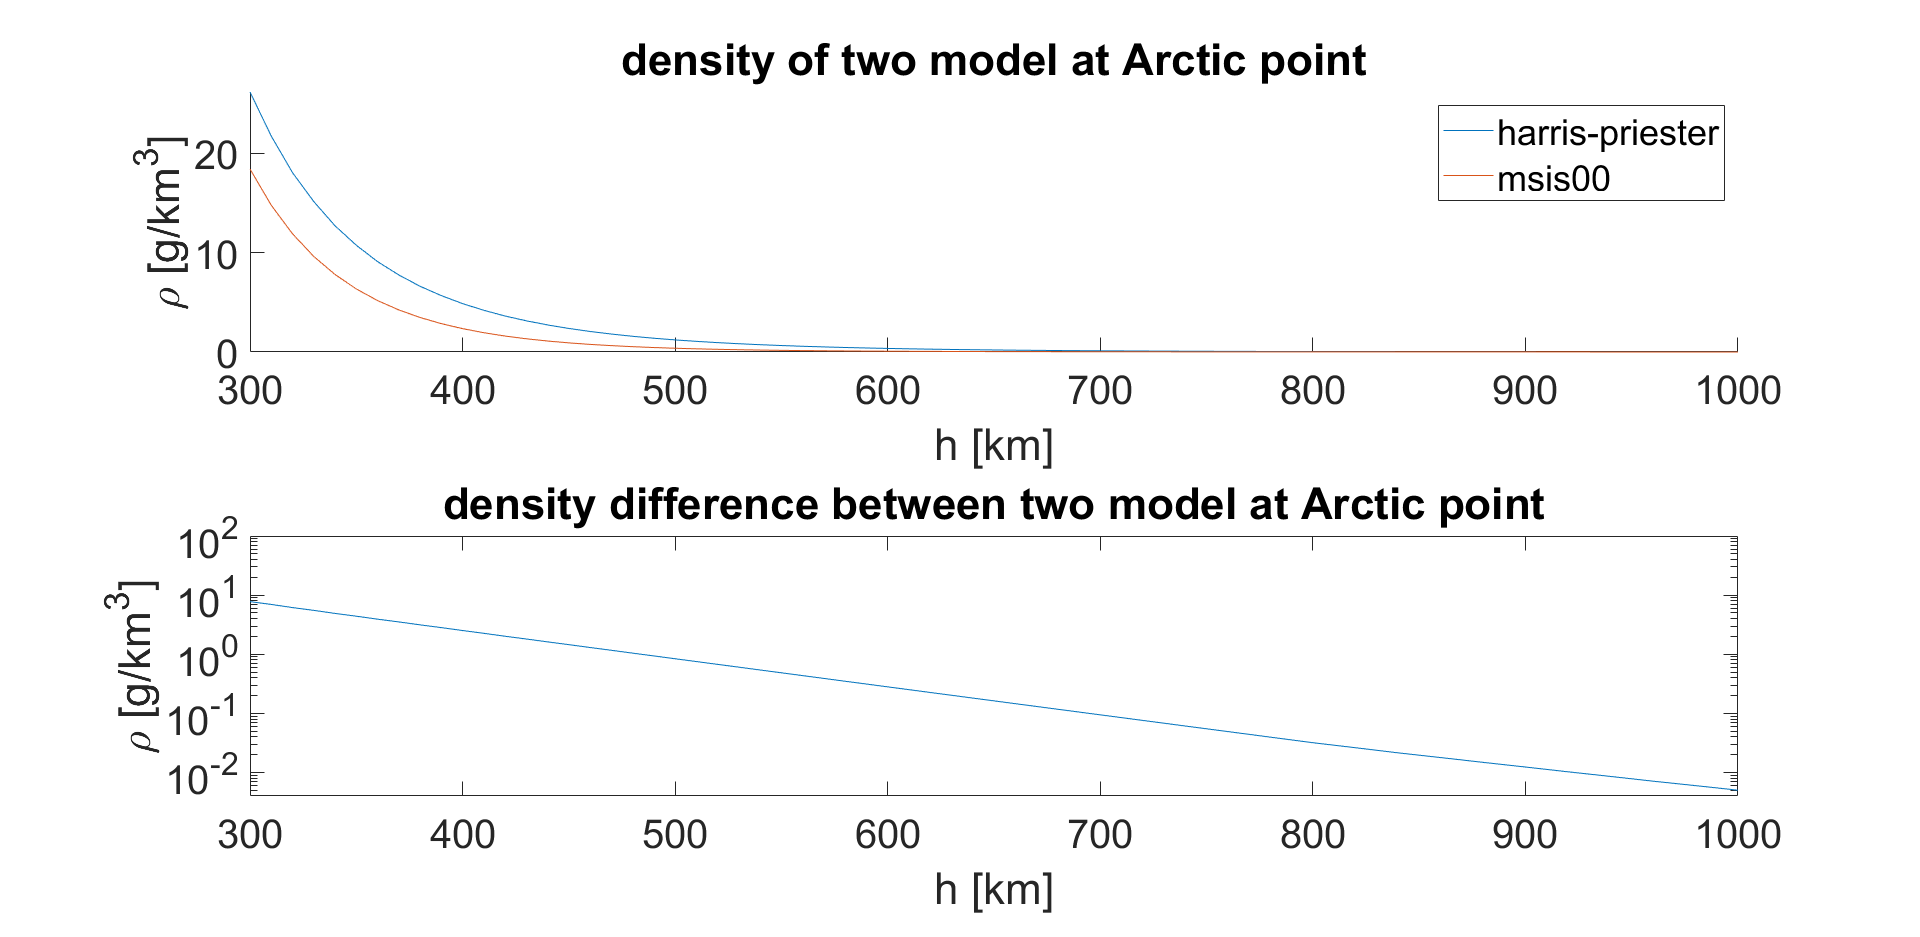
\includegraphics[width=0.9\textwidth]{images/compare_arctic.png}}
	\subfigure[]{
		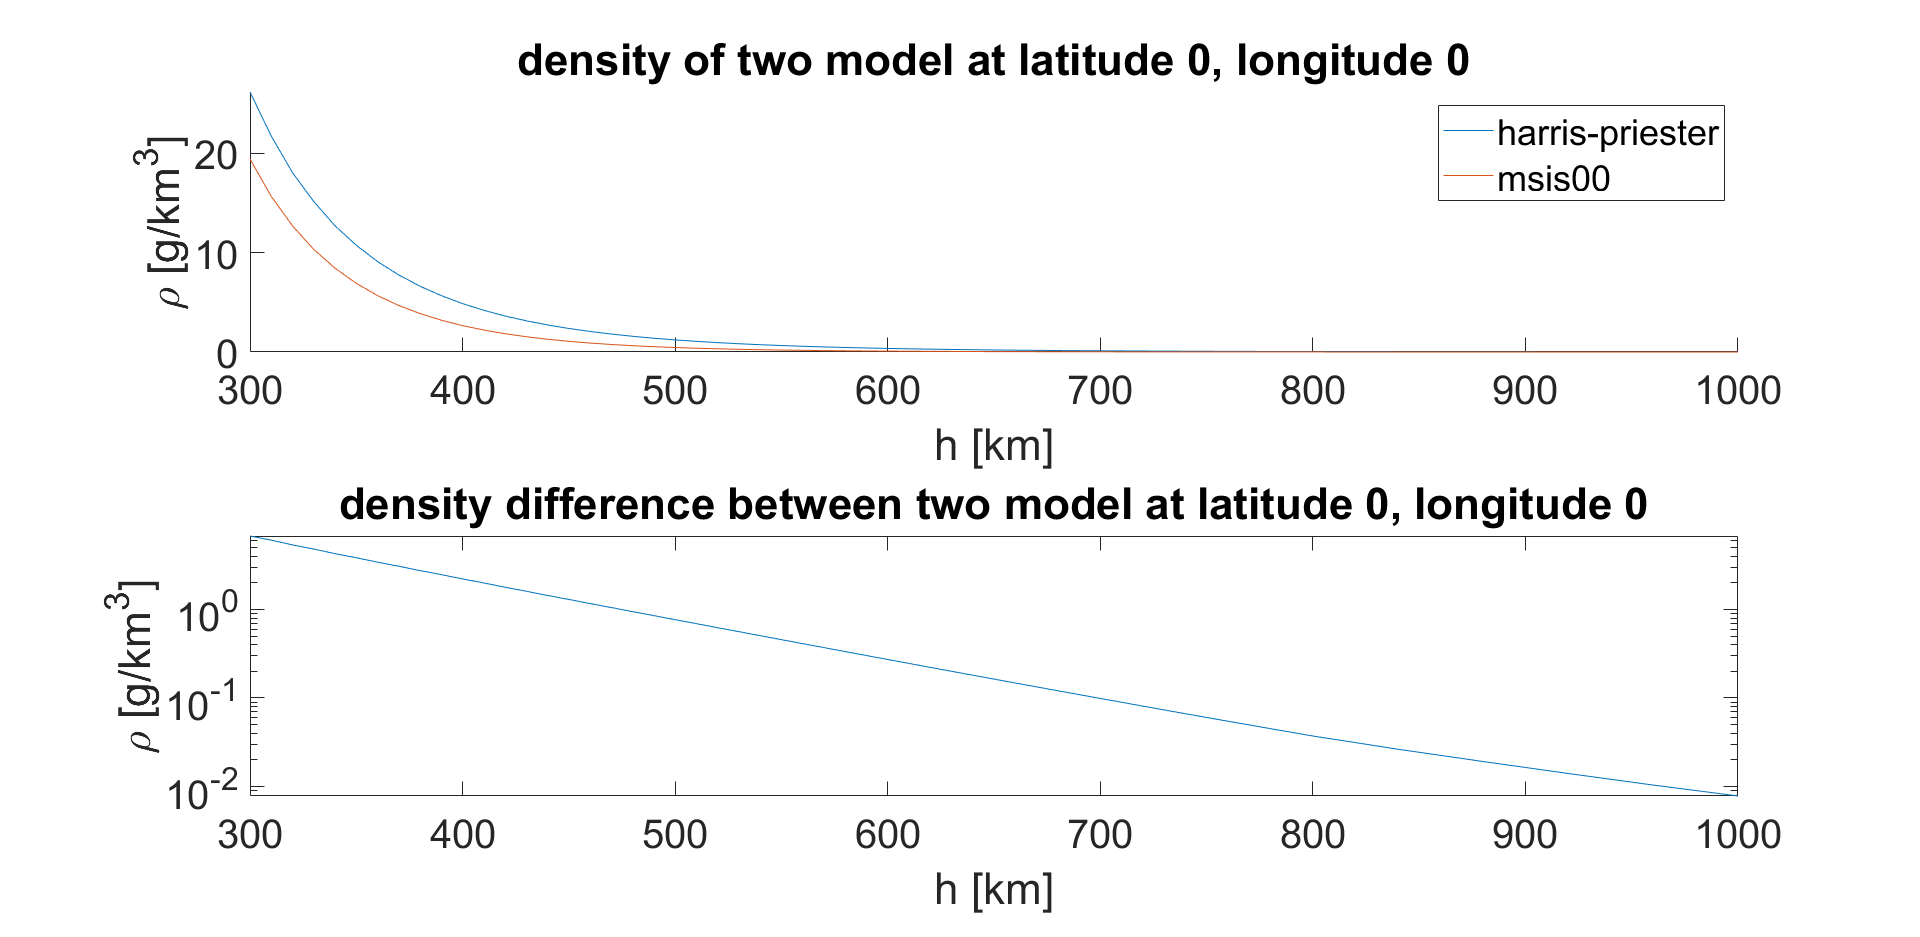
\includegraphics[width=0.9\textwidth]{images/compare_equa.png}}
\end{figure}
\clearpage
\bibliography{bib/bib.bib}
\end{document}



